\documentclass[14pt]{extarticle}
\usepackage{amsmath}
\usepackage{amssymb}
%\usepackage{tikz}
%\usetikzlibrary{calc}
%\usetikzlibrary{trees}
\usepackage{hyperref}
\usepackage{graphicx}
\graphicspath{ {../../chap10/} }
\usepackage[top=0.75in, bottom=0.75in, left=0.75in, right=0.75in]{geometry}
%\newcommand*{\Scale}[2][4]{\scalebox{#1}{\ensuremath{#2}}}%
\usepackage[shortlabels]{enumitem}
\usepackage[most]{tcolorbox}
\definecolor{bg}{RGB}{255,249,227}
% \usepackage{showframe}

\title{\vspace{-5ex}Math 208 Section 10.1, 10.2}
\date{\vspace{-10ex}}
\usepackage{multicol}
\setlength{\columnsep}{1cm}
\setlength{\parindent}{0pt}
\usepackage{parskip}
\setlength{\parskip}{10pt} % 1ex plus 0.5ex minus 0.2ex}
%\usepackage{ragged2e}


\begin{document}
	\maketitle		
	\section*{Homework, Reading, and Other}
	\begin{itemize}
		\item Section 10.1
		\item Section 10.2
	\end{itemize}

\section{Section 10.1: e}
\subsection{Goals}
\begin{itemize}
	\item Recall and understand basics of $e$
	\item Solve continuous compounding questions
\end{itemize}
\subsection{Detail}
One  of the most important numbers in math is $e$. You will come across it often, it is very useful, and it has some very interesting properties.
\begin{align*}
	&e = \lim_{n \to \infty} \left(1 + \frac{1}{n}\right)^n &
	\textbf{ or } &
	&e = \lim_{s \to 0} \left(1 + s\right)^{\frac{1}{s}}
\end{align*}
It is often used for modeling continuous growth. It is the base for the natural logarithm and an its slope is equal to its value.
\begin{align*}
	\frac{d}{dx}e^x =  e^x
\end{align*}
Some additional properties:
\begin{align*}
	&e^0 = 1 & &e^{x+y} = e^x e^y & &e^{-x}=\frac{1}{e^x} \\
	&e^{x-y} = \frac{e^x}{e^y }	& &(e^x)^r= e^{rx} & &\ln(e^x) = x
\end{align*}
		

We have already seen it used in continuous compounding, where:
\begin{align*}
	A = Pe^{rt}
\end{align*}

\subsection{Examples}
\begin{center}
	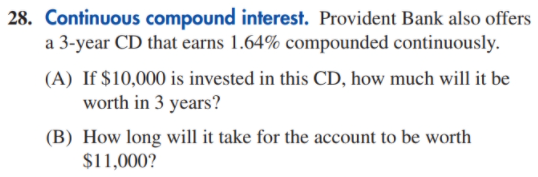
\includegraphics[width=0.75\linewidth]{10-1-28}
\end{center}
(A) Using $A = Pe^{rt}$.
\begin{align*}
	A &= 10000e^{.0164(3)} \\
	&=\$10504.30
\end{align*}
(B) Starting with $A = Pe^{rt}$.
\begin{align*}
	A/P &= e^{rt} \\
	\ln(A/P)&=rt \\
	t &= \frac{1}{r} \ln(\frac{A}{P}) \tag{1}\\
	&= \frac{1}{.0164} \ln(\frac{11000}{10000}) \\
	&\approx 5.8 \text{ years}
\end{align*}
(C) How long will it take for the investment to triple?

To triple means that $A$ is three times $P$ or $A/P = 3$. Starting with equation (1), we have 
\begin{align*}
	t &= \frac{1}{r} \ln(\frac{A}{P}) \\
	&= \frac{1}{.0164} \ln(3) \\\\
	t&\approx 67 \text{ years}
\end{align*}

\subsection{Homework}
27, 29, 31,35, 43


\cleardoublepage
\section{Section 10.2: Derivative of Exponential and Logarithm}

\subsection{Inverses}
An inverse function is a function that "reverses" the operations of another function. As an example, let $f(x) = 3x-2$. In this function, we take a value of $x$ and multiply it by 3, then we subtract 2 from that result. To reverse the function, we take a value of $y$ and add 2 to it and then divide that result by 3. Thus $f^{-1}(y) = \frac{1}{3}(y+2)$

In the case of $e^x$, we have that its inverse is $ln(x)$.
\begin{center}
	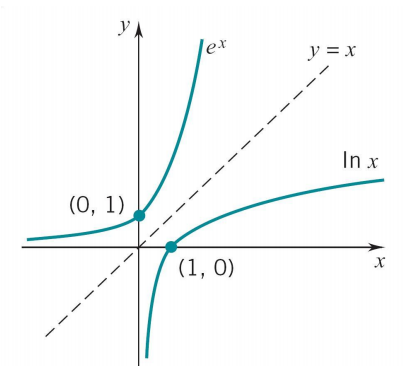
\includegraphics[width=0.5\linewidth]{10-2-1}
\end{center}
Then
\begin{align*}
	&\ln(e^x) = x & & \text{and} & &e^{\ln(x)} = x 
\end{align*}
\subsection{Derivatives}
You CANNOT use the power rule to find the derivative of $e^x$. Instead we must use the definition. This requires some mathematics of series which we have not covered. So, without proving, we have
\begin{tcolorbox}[enhanced jigsaw,colback=bg,boxrule=0pt,arc=0pt]
	\textbf{Exponential and Logarithm Derivatives}
	\begin{align*}
		&\frac{d}{dx}e^x =  e^x & &(\text{for all } x) \\\\
		&\frac{d}{dx}\ln(x) =  \frac{1}{x} & &(\text{for } x>0)
	\end{align*}
\end{tcolorbox}

\subsection{Logarithm rules}
Generally, logarithm means the natural logarithm or log base e, unless otherwise indicated.
\begin{tcolorbox}[enhanced jigsaw,colback=bg,boxrule=0pt,arc=0pt]
	\textbf{Properties of Logarithms} If b, M, and N are positive real numbers, $b \neq 1$, and p and x are real numbers, then
	\begin{align}
		&\log_b(1)=0 \\
		&\log_b(b)=1 \\
		&\log_b(b^x)=x \\
		&b^{\log_b(x)}=x, \text{ when }x> 0 \\
		&\ln(MN) = \ln(M) + \ln(N) \\ 
		&\ln(M/N)=\ln(M)-\ln(N) \\
		&\ln(N^p)= p\ln(M) \\ 
		&\ln(M) = \log_e(M)
	\end{align}
\end{tcolorbox}
\begin{tcolorbox}[enhanced jigsaw,colback=bg,boxrule=0pt,arc=0pt]
	\textbf{Properties of e} If p and x are real numbers, then
	\begin{align}
		&e \approx 2.71828 \cdots \\
		&e^0 = 1 \\
		&e^{x+y} = e^x e^y  \\
		&e^{-x}=\frac{1}{e^x} \\
		&e^{x-y} = \frac{e^x}{e^y } \\ 
		&(e^x)^p= e^{px} \\
		&\ln(e^x) = x 
	\end{align}
\end{tcolorbox}

\subsection{Examples}
Find the derivative
\begin{enumerate}
	\item (14) $f(x)= -7e^x - 2x+5$. \\
	Using the Sum and Difference Property, we find the derivative of each term.\\
	$$f'(x) = -7e^x -2$$
	
	\item (22) $f(x) = \ln(x^8)$. \\
	First, we use logarithm properties to rearrange and then find the derivative. \\
	\begin{align*}
		f(x) &= 8\ln(x) \\
		f'(x) &= \frac{8}{x}
	\end{align*}

	\item $f(x) = 3x^e$. \\
	Recall that $e$ is a constant. Then $$f'(x) = 3ex^{e-1}=3ex^ex^{-1} = \frac{3ex^e}{x}$$
	
	\item (29) $f(x) = xx^e$. \\
	Recall again the $e$ is a constant. We first rearrange and then solve
	\begin{align*}
		f(x) &= x^1x^e = x^{e+1} \\
		f'(x) &= (e+1)x^{e+1-1} = (e+1)x^e
	\end{align*}
	
	\item (30) $f(x) = ee^x$. \\
	Recall again the $e$ is a constant. $$f'(x)= ee^x$$
	
	\item $f(x) = \ln\left(\frac{x^2}{e}\right)$\\
	First, we use logarithm properties to rearrange and then find the derivative. \\
	\begin{align*}
		f(x) &= \ln(x^2) - \ln(e) = 2\ln(x) - 1 \\
		f'(x) &= \frac{2}{x}
	\end{align*}
\end{enumerate}


\noindent\rule{\textwidth}{1pt}
{\footnotesize Copyright (C) 2021 Garold Dalton --- Released under GNU General Public License v3.0}


\cleardoublepage


\end{document}
